\documentclass[12pt]{article}
\usepackage{lingmacros}
\usepackage{tree-dvips}
\usepackage{multicol}
\usepackage{graphicx}
\usepackage[section]{placeins}
\usepackage{hyperref}
\usepackage{caption}
\usepackage{listings}
\usepackage{indentfirst}


\hypersetup{
	colorlinks=true,
	linkcolor=blue,
	filecolor=magenta,      
	urlcolor=cyan,
}
\title{\Huge \bfseries \emph{Assignment 3}}
\author{Vathana Him}
\date{November 25, 2021}


\begin{document}
\maketitle
\section{Abstract}
\hspace*{5mm} The purpose of this assignment is to use the data of the image created from assignment 1 to build classification models in a distributed system in databricks in order to classify the choosen images
and compare the results and run time to that of the model built in our local machine. This assignment utilized images from UCI respository as sample datasets that will be used to train a machine learning model. 
Images that were processed represented three fruits spanish pear, fuji apple, watermelon. These images were labeled as Image0, Image1, and Image2 respectively and their dataset was processed and dervied in assignment1 for both the non-overlapping and 
overlapping layer. These labels was then encoded to take in the values of 0, 1, and 2. The primary machine learning that was used in order to classify these images was random forest. Prior to training the machine learning model,
additional methods were taken into account in feature selection and data scaling in order to reduce the size of the data and train the model with a sufficient outcome.
The random forest model in databricks was then used to compare to the random forest model that was dervied in our local machine in assignment2. 

\begin{multicols*}{2}
  \section{Task 1}
  \hspace*{5mm} In assignment1, the three images were divided into 8X8 pixel blocks, the grayscale images were then divided into sliding block of 8X8 pixels. Each feature was then assigned a label respectively to identify them. 
  Two helper functions were used for this task, sliding blocks feature function which converts an image into sliding image blocks given an image object, and 
  label feature function which create feature labels for each image given a list that contains the array of sliding images. The dimension of the gray images were resized to height of 256 and width of 344. The purpose for these choosen dimensions was to keep its aspect ratio. 
  Additionally, the resized height and width must also be divible by eight since this project divided the targeted image into sliding blocks and non-sliding blocks of 8 by 8 height and width. T
  he feature vector that was constructed from these images created 3400 feature vectors for the sliding block and 1600 feature vectors for the non-sliding block and each feature vector lies a 8 by 8 pixels who’s value lies between 0-255 of the gray image scale. 
  The features of each feature vector was then flatten to 64 features for each respective feature vector. These datasets was exported into cvs files in the data folder.
  The evidence of this dataset can be shown in 2.1 Figure 1. 

  \subsection{Assignment 1 Figure} 
	\begin{center}
		\captionof{figure}{CVS Data Folder}
		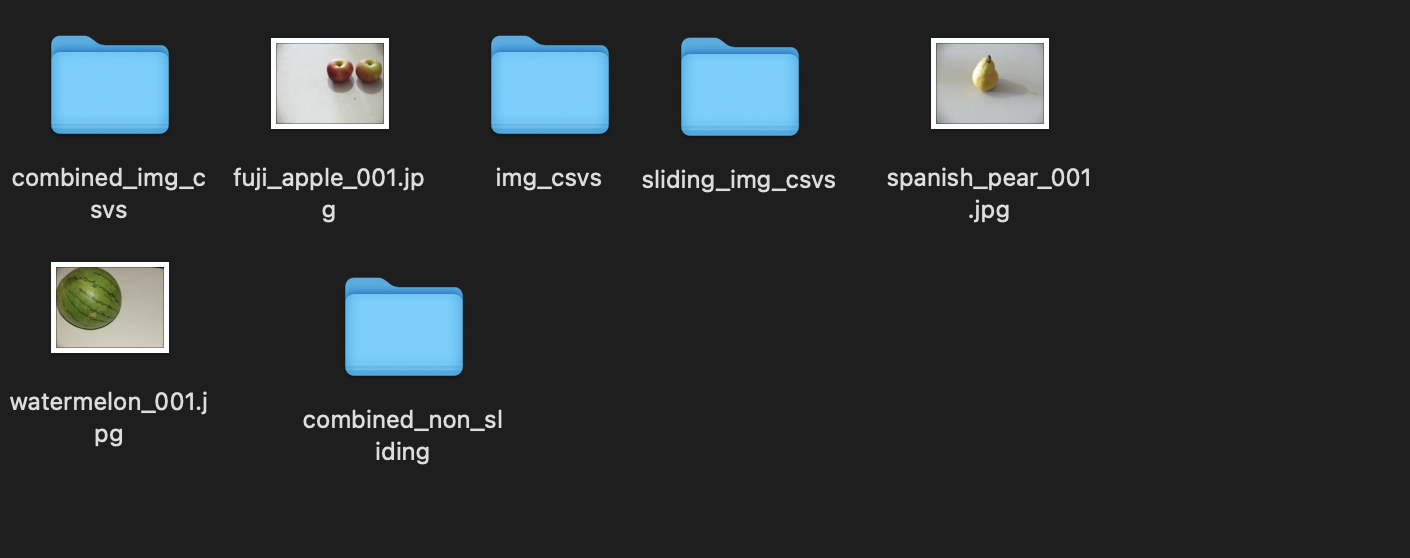
\includegraphics[scale=0.2]{../screenshot/csvs.png}	
    \end{center}


  \hspace*{5mm} In assignment2, the random forest classifier was used to classify the images of different set in non-overlapping image01, 
  overlapping image01, non-overlapping image012, and overlapping image012. Feature selection was also used in this model to increase
  the speed of the training time and reduce the computational power. The select from model feature selection from Sklearn compare the average
  importance of all features at a threshold value and dropped features that were below the threshold. Additionally the elastic net model will also be presented. However, the random forest models
  will only be used to compare with the databricks model. 

  \hspace*{5mm} In the two class classification for non-overlapping image0 and image1, the training accuracy score was 0.95 and the testing 
  accuracy score was 0.92 based on 2.2 Figure 2. There was not a significant difference between the train and test score, this suggests that the train-test split 
  provided a well balanced data between the two classes. The confusion matrix in 2.2 Figure 3 confirmed a true prediction value of 240 and false prediction value of 
  32 for class 0 and a true prediction value of 269 and false prediction value of 10 for class 1. This indicate that the accuracy rate and the precision
  rate for class 0 and class 1 was relatively as seen in 2.2 Figure 4 of the derived accuracy score and precision for both class 0 and class 1 respectively.
  Class 0 had a precision rate of 0.92, while class 1 had a precision rate of 0.89. This model provided a good accruacy for each of the predicted classes.

  \subsection{Assignment 2 Figure} 
  \begin{center}
      \captionof{figure}{Non-Overlapping Image01 RF Score}
		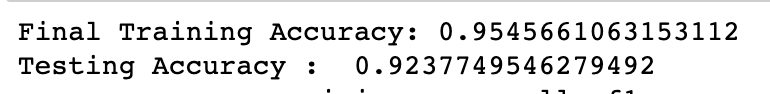
\includegraphics[scale=0.5]{../screenshot/Rf-Non-Overlapping01/score.png}

        \captionof{figure}{Non-Overlapping RF Confusion-Matrix}
            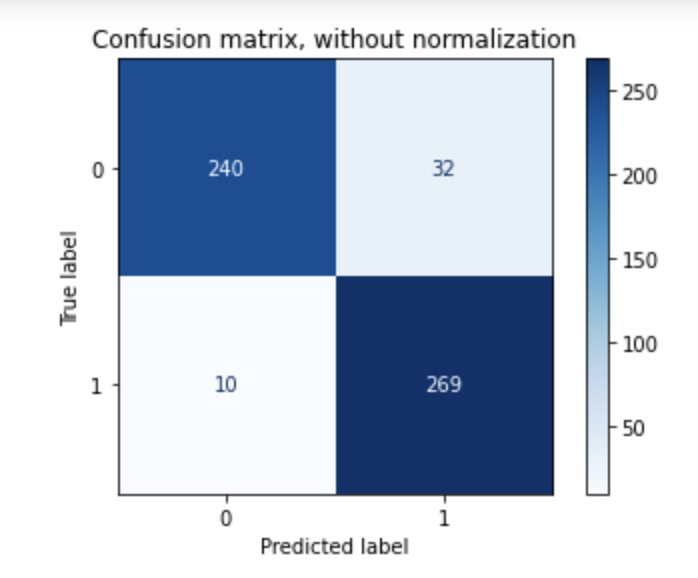
\includegraphics[scale=0.5]{../screenshot/Rf-Non-Overlapping01/cf.png}

        \captionof{figure}{Non-Overlapping RF Derived Score}
        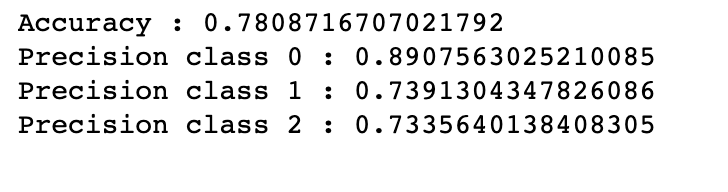
\includegraphics[scale=0.5]{../screenshot/Rf-Non-Overlapping012/calc_score.png}
  \end{center}

  \hspace*{5mm} For the overlapping two-class classificaion of image0 and image1, the training accruacy score was ~0.96 and the testing
  accuracy score was 0.92 based on 2.3 Figure 5. This small difference in accuracy score indicates that the train-test split provided an evenly balanced data for the test and train
  set for the random forest model. The confusion matrix on 2.3 Figure 6 provided the result of the test set as class 0 had 590 true prediction and 74 false prediction,
  while class 1 had 666 true prediction and 30 false prediction. This indicated a high precision value for both class 0 and class 1 because the model
  was able to make a prediction of the two images at a high accuracy rate. Based on the value of this confusion matrix, the hand calculation for accuracy score,
  precision for class 1 and precision for class 0 was derived. In 2.3 Figure 7, the accuracy score from the dervied calculation was 0.92 with a precision of 0.95 and 0.9
  for class 0 and class 1 respectively. Based on these high precision values, it indicated that this model can be produced the same results when test with another
  dataset of the same characteristics. This model also performed significantly better than the elstaic-net for two-class classification of overlapping
  image0 and image1. 

  \subsection{Assignment 2 Figure} 
  \begin{center}
        \captionof{figure}{Over-lapping Image01 RF Score}
        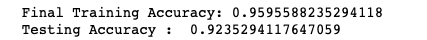
\includegraphics[scale=0.5]{../screenshot/Rf-Overlapping01/score.png}

        \captionof{figure}{Over-lapping RF Confusion-Matrix}
        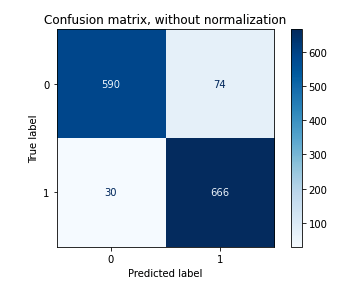
\includegraphics[scale=0.5]{../screenshot/Rf-Overlapping01/cf.png}

        \captionof{figure}{Over-lapping RF Derived Score}
        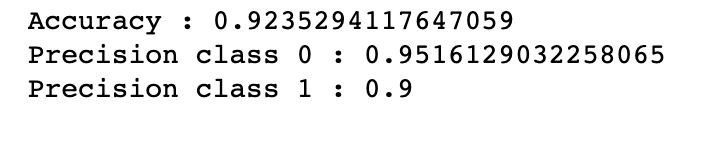
\includegraphics[scale=0.5]{../screenshot/Rf-Overlapping01/calc_score.png}

  \end{center}

  \hspace*{5mm} In the non-overlapping elastic model, the data for non-overlapping image01 was used. The result of the model for
  non-overlapping image01 yielded a training accuracy of 0.69 and testing accuracy of 0.67 as shown in 2.4 Figure 8. A similar 
  score in both the train and test set indicate that the data was balanced between the train and test set. The confusion matrix in 2.4 
  Figure 9 indicate that there were 197 predictions of True Positive for class 0 and 175 predictions of True Positive for class 1. These
  results was then used to manually derived the accuracy and precision. According to the manual derivated result in 2.4 Figure 10, the overall
  accuracy of the model was 0.72 with a precision of 0.72 for class 0 and 0.72 for class 1. This accuracy score indicate that there was a sufficient
  number of true postives for class 0 and class 1. However, the number of false postives was still indicative in affecting the accuracy score.


  \subsection{Assignment 2 Figure} 
  \begin{center}

    \captionof{figure}{Non-Overlapping Image01 Elastic-Net}
    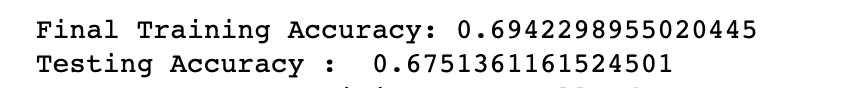
\includegraphics[scale=0.5]{../screenshot/Non-Overlapping-Elastic-results/results.png}

    \captionof{figure}{Non-Overlapping Image01 Elastic-Net Confusion-Matrix}
    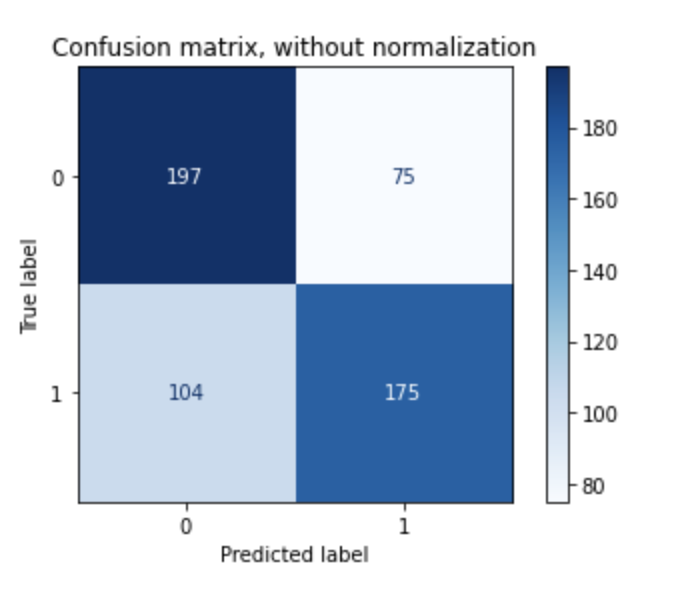
\includegraphics[scale=0.5]{../screenshot/Non-Overlapping-Elastic-results/cf.png}

    \captionof{figure}{Non-Overlapping Image01 Elastic-Net Derived Score}
    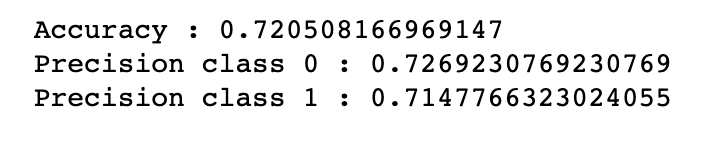
\includegraphics[scale=0.5]{../screenshot/Non-Overlapping-Elastic-results/calc_score.png}

  \end{center}

  \hspace*{5mm} In the second elastic model, the data for overlapping image01 was used. The result of the model for overlapping
  image01 resulted in a training accuracy of 0.60 and a testing accuracy of 0.59. This inidcated that the data had a great degree of
  randomeses and it was balanced in the train-test set. The confusion matrix in 2.5 Figure 11 resulted in 493 prediction of true prediction 
  and 314 of true prediction for class 0 and 1 respectively. However, in the derived precision score for class 0 was relatively lower than that
  of class 1 as shown in 2.5 Figure 12. This could indicate that there was an imbalance in the dataset between class 0 and class 1. Additionally, because of the nature of the
  image choosen, the black and white image of apple and pear had similar texture and texture. The overlapping nature of the dataset could distort the elastic-net loss function, 
  when it attempted to classify the two images. This also impacted the overall dervied accuracy score of the model with a value of 0.65 as shown in 
  2.5 Figure 13. An accuracy score of 0.65 indicate that this model was not sufficient enough for making a prediction. 


  \subsection{Assignment 2 Figure} 
  \begin{center}

    \captionof{figure}{Overlapping Image01 Elastic-Net}
    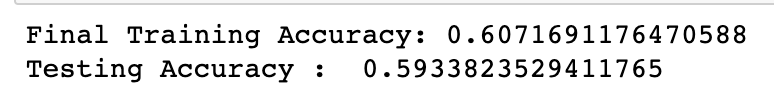
\includegraphics[scale=0.5]{../screenshot/Overlapping-Elastic-results/results.png}

    \captionof{figure}{Overlapping Image01 Elastic-Net Confusion-Matrix}
    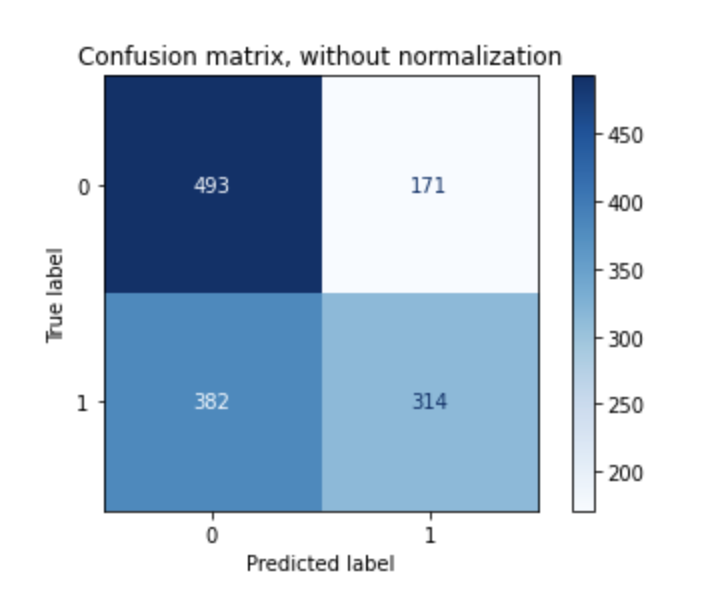
\includegraphics[scale=0.5]{../screenshot/Overlapping-Elastic-results/cf.png}

    \captionof{figure}{Overlapping Image01 Elastic-Net Derived Score}
    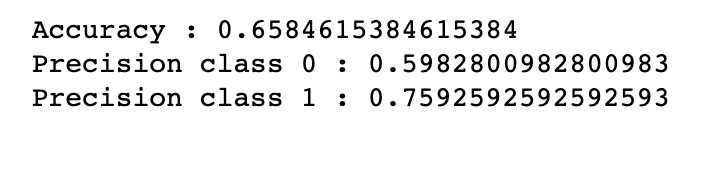
\includegraphics[scale=0.5]{../screenshot/Overlapping-Elastic-results/hand_score.png}

  \end{center}

  \hspace*{5mm} In contrast to the two-class non-overlapping classification random forest, the three-class
  classification of image0, image1 and image2 testing and training accuracy score deviate in larger degree.
  In 2.6 Figure 14, the training accuracy for this model is 0.89, whereas the testing accuracy for this model is 
  0.78. This may indicate an overfit in the model and that the train-test split set did not generate a well balanced enough data.
  The confusion matrix in 2.6 Figure 15 showed that a true prediction value of 212 for class 0, 221 for class 1, and 212 for class 2.
  These values was then used to dervied the caculated precision for each of the class. 2.6 Figure 16 indicated that class 0 had a 0.89 precision,
  class 1 had a precision of 0.74 and class 2 ha da precision of 0.73. The difference in this precision score can suggest that the model
  was overfitted to favor class 0. 


  \subsection{Assisgnment 2 Figures} 
	\begin{center}
    \captionof{figure}{Non-Overlapping Image012 RF Score}
		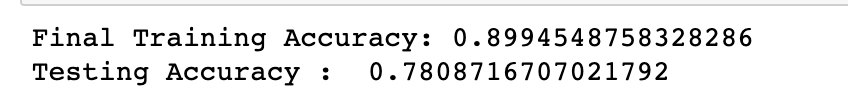
\includegraphics[scale=0.5]{../screenshot/Rf-Non-Overlapping012/score.png}

    \captionof{figure}{Non-Overlapping Image012 RF Confusion-Matrix}
		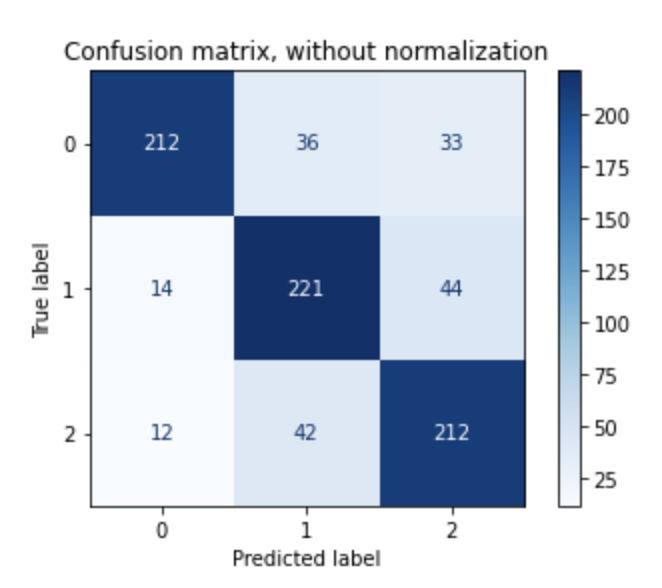
\includegraphics[scale=0.5]{../screenshot/Rf-Non-Overlapping012/cf.png}

    \captionof{figure}{Non-Overlapping Image012 RF Derived Score}
		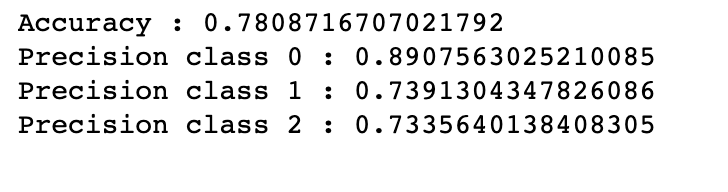
\includegraphics[scale=0.5]{../screenshot/Rf-Non-Overlapping012/calc_score.png}
	\end{center}


  \hspace*{5mm} Similar to the three-class non-overlapping random forest model, the three-class classification of overlapping 
  image0, image1 and image2 testing and training accuracy score also deviated to a noticeable extent.
  In 2.7 Figure 17, the training accuracy for this model is 0.91, whereas the testing accuracy for this model is 
  0.83. This may indicate a slight overfit in the model and that the train-test split set did not generate a well balanced enough data.
  The confusion matrix in 2.7 Figure 18 showed that a true prediction value of 552 for class 0, 608 for class 1, and 545 for class 2.
  These values was then used to dervied the caculated precision for each of the class. 2.7 Figure 19 indicated that class 0 had a 0.94 precision,
  class 1 had a precision of 0.77 and class 2 ha da precision of 0.81. The difference in this precision score can suggest that the model
  was overfitted to favor class 0, which is similar to that of the three-class random forest non-overlapping model. Although the dataset was 
  randomly shuffled, the training set may have contained slightly more data for class 0 than that of class 2 and class 1.  

  \subsection{Assisgnment 2 Figures} 
  \begin{center}
    \captionof{figure}{Overlaping Image012 RF Score}
		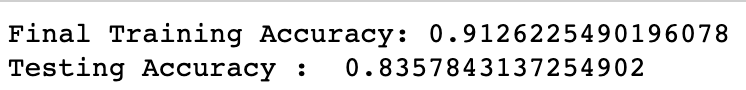
\includegraphics[scale=0.5]{../screenshot/Rf-Overlapping012/score.png}

    \captionof{figure}{Overlapping Image012 RF Confusion-Matrix}
		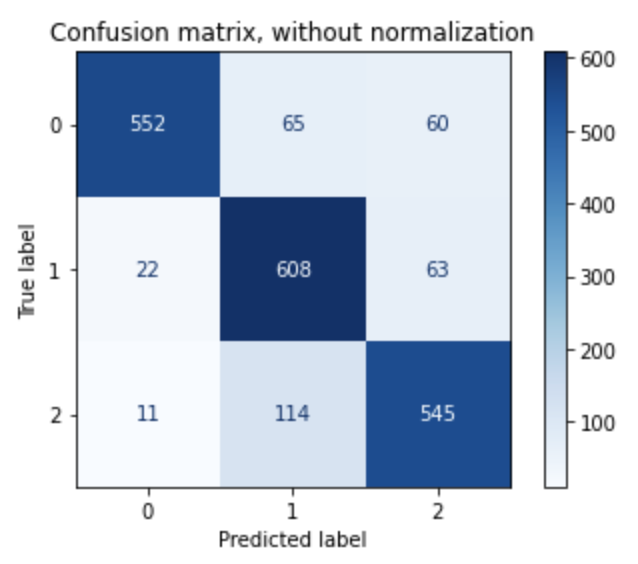
\includegraphics[scale=0.5]{../screenshot/Rf-Overlapping012/cf.png}

    \captionof{figure}{Overlapping Image012 RF Derived Score}
		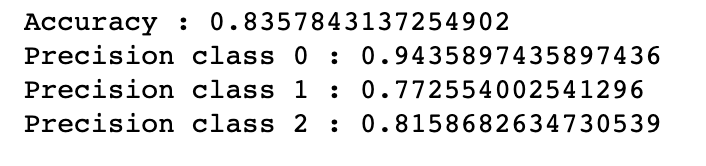
\includegraphics[scale=0.5]{../screenshot/Rf-Overlapping012/calc_result.png}
  \end{center}


\end{multicols*}

		

	

\end{document}